% Build: make
% Timing and sources are in outline.md.
\documentclass[aspectratio=169,11pt]{beamer}
\usetheme{metropolis}
\metroset{progressbar=frametitle,numbering=fraction}
\setbeamertemplate{navigation symbols}{}
\usefonttheme{professionalfonts}
\usefonttheme[onlymath]{serif}
\usepackage[T1]{fontenc}
\usepackage{lmodern}
\usepackage{amsmath,amssymb,mathtools,stmaryrd,booktabs,appendixnumberbeamer,tikz}
\usetikzlibrary{arrows.meta,positioning}
\definecolor{Navy}{HTML}{15324F}
\definecolor{Teal}{HTML}{007F82}
\definecolor{Gold}{HTML}{D48B18}
\definecolor{Pale}{HTML}{EAF4F4}
\setbeamercolor{frametitle}{bg=Navy,fg=white}
\setbeamercolor{progress bar}{fg=Teal,bg=black!12}
\setbeamercolor{alerted text}{fg=Teal}
\setbeamercolor{block title}{bg=Pale,fg=Navy}
\setbeamercolor{block body}{bg=Pale!55,fg=Navy}
\setbeamerfont{frametitle}{size=\large}
\setbeamersize{text margin left=9mm,text margin right=9mm}
\newcommand{\F}{\mathbb{F}}
\newcommand{\RM}{\operatorname{RM}}
\newcommand{\wt}{\operatorname{wt}}
\newcommand{\sw}{\operatorname{sw}}
\newcommand{\supp}{\operatorname{supp}}
\newcommand{\CCZ}{\operatorname{CCZ}}
\newcommand{\ket}[1]{\lvert #1\rangle}
\newcommand{\qcode}[3]{\llbracket #1,#2,#3\rrbracket}
\newcommand{\takeaway}[1]{\vfill\begin{beamercolorbox}[sep=1ex,wd=\linewidth]{block body}#1\end{beamercolorbox}}
\newcommand{\source}[1]{\par\smallskip{\scriptsize\color{black!55}#1\par}}
\newcommand{\storypart}[1]{\setbeamertemplate{frame footer}{\color{Teal}#1}}
\setbeamercovered{invisible}
\newcommand{\talktext}{\small\setlength{\parskip}{2.5pt}\setlength{\abovedisplayskip}{5pt}\setlength{\belowdisplayskip}{5pt}\setlength{\abovedisplayshortskip}{3pt}\setlength{\belowdisplayshortskip}{3pt}}
\newcommand{\threechoices}[3]{%
\begin{center}
\begin{tikzpicture}[node distance=6mm]
\node[fill=Pale,align=center,text width=3.3cm,minimum height=10mm,font=\small] (a) {#1};
\node[fill=Pale,align=center,text width=3.3cm,minimum height=10mm,font=\small,right=of a] (b) {#2};
\node[fill=Pale,align=center,text width=3.3cm,minimum height=10mm,font=\small,right=of b] (c) {#3};
\draw[-{Stealth},Teal,thick] (a)--(b);
\draw[-{Stealth},Teal,thick] (b)--(c);
\end{tikzpicture}
\end{center}}
\newcommand{\facepicture}{%
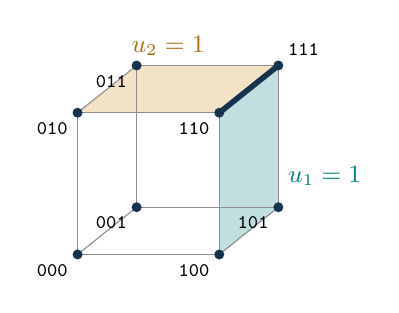
\begin{tikzpicture}[x=1cm,y=1cm]
\foreach \i in {0,1}{\foreach \j in {0,1}{\foreach \k in {0,1}{
 \coordinate (v\i\j\k) at ({1.8*\i+.75*\k},{1.8*\j+.6*\k});
}}}
\fill[Teal!25] (v100)--(v110)--(v111)--(v101)--cycle;
\fill[Gold!25] (v010)--(v110)--(v111)--(v011)--cycle;
\foreach \j in {0,1}{\foreach \k in {0,1}{\draw[black!45] (v0\j\k)--(v1\j\k);}}
\foreach \i in {0,1}{\foreach \k in {0,1}{\draw[black!45] (v\i0\k)--(v\i1\k);}}
\foreach \i in {0,1}{\foreach \j in {0,1}{\draw[black!45] (v\i\j0)--(v\i\j1);}}
\draw[Navy,line width=2pt] (v110)--(v111);
\foreach \i in {0,1}{\foreach \j in {0,1}{\foreach \k in {0,1}{\fill[Navy] (v\i\j\k) circle[radius=1.8pt];}}}
\node[right,text=Teal,font=\small] at (2.55,1) {$u_1=1$};
\node[above,text=Gold!80!black,font=\small] at (1.15,2.4) {$u_2=1$};
\foreach \i in {0,1}{\foreach \j in {0,1}{\foreach \k in {0,1}{
\pgfmathtruncatemacro{\vertexsum}{\i+\j+\k}
\ifnum\vertexsum=3
\node[above right,font=\scriptsize] at (v\i\j\k) {$\mathtt{\i\j\k}$};
\else
\node[below left,font=\scriptsize] at (v\i\j\k) {$\mathtt{\i\j\k}$};
\fi
}}}
\end{tikzpicture}}
% Corruption: 0 clean, 1 marked, 2 unmarked. Second argument highlights u1 edges.
\newcommand{\cubepicture}[3]{%
\begin{tikzpicture}[x=1.05cm,y=1.05cm]
\foreach \i in {0,1}{\foreach \j in {0,1}{\foreach \k in {0,1}{
  \coordinate (v\i\j\k) at ({1.9*\i+.85*\k},{1.9*\j+.7*\k});
}}}
\foreach \j in {0,1}{\foreach \k in {0,1}{
  \ifnum#2=1 \draw[Gold,line width=2pt] (v0\j\k)--(v1\j\k);
  \else \draw[black!40,thick] (v0\j\k)--(v1\j\k);\fi
}}
\foreach \i in {0,1}{\foreach \k in {0,1}{\draw[black!40,thick] (v\i0\k)--(v\i1\k);}}
\foreach \i in {0,1}{\foreach \j in {0,1}{\draw[black!40,thick] (v\i\j0)--(v\i\j1);}}
\foreach \i in {0,1}{\foreach \j in {0,1}{\foreach \k in {0,1}{
  \pgfmathtruncatemacro{\bit}{mod(\i+\j+\k,2)}
  \pgfmathtruncatemacro{\origin}{\i+\j+\k}
  \ifnum#1>0\ifnum\origin=0\def\bit{1}\fi\fi
  \ifnum\bit=1\def\fillcolor{Teal}\def\textcolor{white}
  \else\def\fillcolor{white}\def\textcolor{Navy}\fi
  \ifnum#3=1
    \ifnum\bit=1\def\nodetext{$T^\dagger$}\else\def\nodetext{$T$}\fi
  \else\edef\nodetext{\bit}\fi
  \node[circle,draw=Navy,fill=\fillcolor,text=\textcolor,minimum size=7.5mm,inner sep=0pt,font=\small] at (v\i\j\k) {\nodetext};
  \node[below=4.3mm,font=\scriptsize,text=Navy] at (v\i\j\k) {$\mathtt{\i\j\k}$};
  \ifnum#1=1\ifnum\origin=0\draw[Gold,line width=1.4pt] (v\i\j\k) circle[radius=4.6mm];\fi\fi
}}}
\end{tikzpicture}}
% Three blocks, with the paper's Gray-order rows u1u2 and columns u3u4.
\newcommand{\blockpicture}[1]{%
\begin{tikzpicture}[x=.63cm,y=.57cm]
\foreach \b/\wa/\wb/\cnt in {0/1/0/6,1/0/1/6,2/1/1/10}{
 \node[text=Navy] at ({5.3*\b+1.5},1.1) {$w=(\wa,\wb)$};
 \foreach \r/\ua/\ub in {0/0/0,1/0/1,2/1/1,3/1/0}{
  \foreach \c/\uc/\ud in {0/0/0,1/0/1,2/1/1,3/1/0}{
   \ifnum#1=1
    \pgfmathtruncatemacro{\flip}{mod(\uc+\wa*(\ua+\ub+\uc+\ua*\uc+\ub*\uc+\ub*\ud)+\wb*(\uc+\ud+\ua*\ub+\ua*\ud+\uc*\ud),2)}
    \ifnum\flip=1\def\shade{Teal!22}\def\gate{$T^\dagger$}\else\def\shade{Gold!18}\def\gate{$T$}\fi
    \node[rectangle,fill=\shade,minimum width=5.9mm,minimum height=5.3mm,font=\scriptsize] at ({5.3*\b+\c},-\r) {\gate};
   \else\fill[Teal] ({5.3*\b+\c},-\r) circle[radius=2.2pt];\fi
  }
 }
 \ifnum#1=1\node[font=\small] at ({5.3*\b+1.5},-4) {$\cnt\ T^\dagger$};
 \else\node[font=\small] at ({5.3*\b+1.5},-4) {$16$ points};\fi
}
\end{tikzpicture}}
\title{Boolean functions: applications in quantum error correction and beyond}
\author{Bohan Lu}
% \institute{Duke University}
\date{Sep 16}
\begin{document}
\begin{frame}[plain,noframenumbering]
\vfill
{\LARGE\bfseries\color{Navy}Boolean functions:\par}
{\Large\bfseries\color{Navy}applications in quantum error correction and beyond\par}
\vspace{9mm}
{\large Bohan Lu\quad Duke University\par}
\vfill
\note{The talk begins with error-correcting computer memory, then constructs the complete eight-bit teaching example before using the same Boolean functions in a quantum calculation.}
\end{frame}

% 1: 1.5 min
\storypart{1 / 3\quad Classical encoding}
\begin{frame}{Correcting one bit of error in memory}
\talktext
\begin{center}
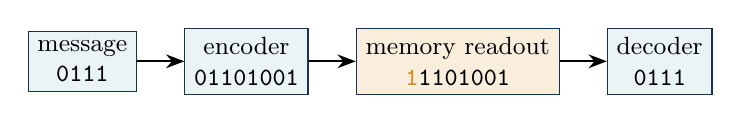
\begin{tikzpicture}[node distance=6mm,font=\small]
\node[draw=Navy,fill=Pale,align=center] (a) {message\\$\mathtt{0111}$};
\node[draw=Navy,fill=Pale,align=center,right=of a] (b) {encoder\\$\mathtt{01101001}$};
\node[draw=Navy,fill=Gold!15,align=center,right=of b] (c) {memory readout\\$\textcolor{Gold}{\mathtt{1}}\mathtt{1101001}$};
\node[draw=Navy,fill=Pale,align=center,right=of c] (d) {decoder\\$\mathtt{0111}$};
\draw[-{Stealth},thick] (a)--(b);
\draw[-{Stealth},thick] (b)--(c);
\draw[-{Stealth},thick] (c)--(d);
\end{tikzpicture}
\end{center}
A memory controller writes an encoded block and checks its constraints when the block is read. A physical disturbance may change a stored $0$ to $1$, or $1$ to $0$.

The \emph{encoder} maps four message bits to eight stored bits. The \emph{decoder} maps the eight values read from memory back to four message bits.

\textbf{Assumption:} at most one stored bit changes, at a position unknown to the decoder.
\takeaway{We will construct all 16 allowed eight-bit words and a decoder that corrects any one changed bit.}
\note{Application context: IBM, \emph{Troubleshooting Memory issues}, states that ECC memory can correct single-bit errors. The eight-bit encoder in this talk is a teaching construction rather than a model of a particular memory product.}
\end{frame}

% 2: 2.5 min
\begin{frame}{The encoder evaluates eight XOR expressions}
\talktext
For bits, $\oplus$ denotes XOR: $0\oplus0=1\oplus1=0$ and $0\oplus1=1\oplus0=1$.
The message is $(b,a_1,a_2,a_3)$. A stored position is an address $u=(u_1,u_2,u_3)$.
The product $a_i u_i$ equals $u_i$ when $a_i=1$ and equals $0$ when $a_i=0$.
\[
f_{a,b}(u)=b\oplus a_1u_1\oplus a_2u_2\oplus a_3u_3.
\]
\begin{center}
\scriptsize
\begin{tabular}{c|cccc}
$u$ & $000$ & $001$ & $010$ & $011$\\\hline
$f_{a,b}(u)$ & $b$ & $b\oplus a_3$ & $b\oplus a_2$ & $b\oplus a_2\oplus a_3$\\
$(b,a_1,a_2,a_3)=(0,1,1,1)$ & $0$ & $1$ & $1$ & $0$
\end{tabular}

\smallskip
\begin{tabular}{c|cccc}
$u$ & $100$ & $101$ & $110$ & $111$\\\hline
$f_{a,b}(u)$ & $b\oplus a_1$ & $b\oplus a_1\oplus a_3$ & $b\oplus a_1\oplus a_2$ & $b\oplus a_1\oplus a_2\oplus a_3$\\
$(b,a_1,a_2,a_3)=(0,1,1,1)$ & $1$ & $0$ & $0$ & $1$
\end{tabular}
\end{center}
Thus the example message is stored as $\mathtt{01101001}$ in address order $000,001,\ldots,111$.
\takeaway{The four message bits still contain all the information. The eight stored values add constraints that make corruption detectable and correctable.}
\end{frame}

% 3: 1.5 min
\begin{frame}{Affine Boolean functions define the codewords}
\talktext
A \emph{Boolean function} maps each binary address to one bit. A constant XOR a binary linear combination of the inputs is an \emph{affine Boolean function}. Thus every message defines the affine function $f_{a,b}$ on the preceding slide.

The \emph{encoder} is the evaluation map
\[
\operatorname{Enc}(b,a_1,a_2,a_3)
=\bigl(f_{a,b}(000),f_{a,b}(001),\ldots,f_{a,b}(111)\bigr).
\]
The message can be recovered from an uncorrupted evaluation word:
\[
b=f_{a,b}(000),\qquad
a_i=f_{a,b}(e_i)\oplus f_{a,b}(000),
\]
where $e_i$ has a $1$ in position $i$ and zeros elsewhere.

Therefore different four-bit messages give different eight-bit words. These $16$ words are the \emph{codewords}, and their set is the code $C$.
\takeaway{$C$ contains 16 selected words among all $2^8=256$ possible eight-bit words.}
\note{Terminology reference: Carlet, \emph{Boolean Functions for Cryptography and Coding Theory}, Section 5.1, ``Affine functions and their combinations.''}
\end{frame}

% 4: 2 min
\begin{frame}{From a truth table to a polynomial}
\talktext
The \emph{algebraic normal form} (ANF) is the unique XOR of products of distinct input variables representing a Boolean function. A product of bits is their AND. The \emph{degree} is the largest number of variables in one nonzero product.

Let $p(u)=u_1\oplus u_2\oplus u_3$ be the encoded example. Let $r$ be the Boolean function whose table is the eight bits read from memory:
\[
p\longleftrightarrow\mathtt{01101001},
\qquad r\longleftrightarrow\mathtt{11101001}.
\]
Only the value at address $000$ changed. Define
\[
\delta_{000}(u)=(1\oplus u_1)(1\oplus u_2)(1\oplus u_3),
\qquad
\delta_{000}(000)=1,\quad \delta_{000}(u)=0\ (u\ne000).
\]
Then
\[
r=p\oplus\delta_{000}
=1\oplus u_1u_2\oplus u_1u_3\oplus u_2u_3\oplus u_1u_2u_3.
\]
\takeaway{Every codeword has degree at most one. The readout has degree three, so $r\notin C$.}
\end{frame}

% 5: 2 min
\begin{frame}{Comparing neighboring table entries}
\talktext
\begin{columns}[c,onlytextwidth]
\column{.32\textwidth}\centering
\resizebox{.79\linewidth}{!}{\cubepicture{1}{1}{0}}
\par\scriptsize Below: address. Teal: $1$. White: $0$. Gold: first-bit edges. Ring: changed entry.
\column{.65\textwidth}
The direction $e_1=(1,0,0)$ toggles the first address bit. The \emph{Boolean derivative} compares the two endpoint values:
\[
D_{e_i}f(u)=f(u\oplus e_i)\oplus f(u).
\]
At the edge containing the changed address,
\[
p(000)\oplus p(100)=0\oplus1=1,
\qquad
r(000)\oplus r(100)=1\oplus1=0.
\]
\begin{center}
\scriptsize
\textbf{Derivatives of $p$ and $r$ along $e_1$.}\\[2pt]
\begin{tabular}{c|cccc}
edge & $000,100$ & $001,101$ & $010,110$ & $011,111$\\\hline
$D_{e_1}p$ & $1$ & $1$ & $1$ & $1$\\
$D_{e_1}r$ & \textcolor{Gold}{$0$} & $1$ & $1$ & $1$
\end{tabular}
\end{center}
\end{columns}
\takeaway{Only the comparison using address $000$ changes. The other three pairs have the same endpoints in $p$ and $r$. The same statement holds in each coordinate direction.}
\end{frame}

% 6: 2 min
\begin{frame}{Recovering the four message coefficients}
\talktext
Toggling $u_i$ cancels every affine term except $a_i u_i$:
\[
D_{e_i}f_{a,b}=a_i.
\]
The four disjoint $e_1$ edges give four estimates of $a_1$:
\begin{center}
\scriptsize
\begin{tabular}{c|cccc}
addresses & $000,100$ & $001,101$ & $010,110$ & $011,111$\\\hline
received XOR & \textcolor{Gold}{$0$} & $1$ & $1$ & $1$
\end{tabular}
\end{center}
\begin{uncoverenv}<2->
One changed address lies on exactly one $e_i$ edge. Hence at least three of the four votes equal $a_i$.
Thus majority gives $a_1=a_2=a_3=1$.
\[
r(u)\oplus a_1u_1\oplus a_2u_2\oplus a_3u_3
\quad\longleftrightarrow\quad \mathtt{10000000}.
\]
Seven entries now equal the constant $b=0$. The decoded message is $(0,1,1,1)$.
\end{uncoverenv}
\vfill
\only<1>{\textbf{Question: Why is this majority reliable?}}
\only<2>{\textbf{Three of four votes recover each $a_i$. Seven residual entries recover $b$.}}
\end{frame}

% 7: 2 min
\begin{frame}{Support intersections compute Hamming distance}
\talktext
For a Boolean function $f$ on the eight addresses, define its support and weight. For two evaluation words, define their \emph{Hamming distance}:
\begin{align*}
\supp(f)&=\{u:f(u)=1\}, & \wt(f)&=|\supp(f)|=\sum_{u\in\F_2^3}f(u),\\
d_H(f,g)&=|\{u:f(u)\ne g(u)\}|, & d_H(f,g)&=\wt(f\oplus g).
\end{align*}
\begin{columns}[c,onlytextwidth]
\column{.32\textwidth}\centering
\resizebox{.61\linewidth}{!}{\facepicture}
\column{.65\textwidth}
The coordinate functions $u_1$ and $u_2$ each have four ones. Their product selects the two addresses on the common edge:
\[
\wt(u_1)=\wt(u_2)=4,\qquad \wt(u_1u_2)=2.
\]
\end{columns}
\[
\wt(f\oplus g)=\wt(f)+\wt(g)-2\wt(fg),
\quad \underbrace{d_H(u_1,u_2)=4+4-2(2)=4}_{\text{one particular pair}}.
\]
\end{frame}

% 8: 2.5 min
\begin{frame}{The code's minimum distance is four}
\footnotesize\setlength{\parskip}{2pt}\setlength{\abovedisplayskip}{3pt}\setlength{\belowdisplayskip}{3pt}
The \emph{minimum distance of the code} is
\[
d_{\min}(C)=\min_{\substack{f,g\in C\\f\ne g}}d_H(f,g).
\]
\begin{columns}[T,onlytextwidth]
\column{.55\textwidth}
For $f\ne g$, $h=f\oplus g$ is nonzero and affine.

If $h$ has coefficient $a_i=1$, each pair $\{u,u\oplus e_i\}$ contains one output $1$. Four pairs give $\wt(h)=4$. The remaining case $h=1$ has weight $8$.

Thus all distinct pairs have distance $4$ or $8$. Slide 7 attains $4$, so $d_{\min}(C)=4$.
\column{.42\textwidth}
For parity $p$, let
\[
H_c=\{u:p(u)=c\}.
\]
Such a level set of a nonzero linear Boolean function is a hyperplane. $H_0$ contains zero. The set
$H_1=\{001,010,100,111\}$ is its translate, an \emph{affine hyperplane}.
\end{columns}
\begin{uncoverenv}<2->
If $f$ and $g$ were each within one change of the same readout $r$, then
\[
4=d_{\min}(C)\le d_H(f,g)
\le d_H(f,r)+d_H(r,g)\le2,
\]
a contradiction. One-error correction is unique.
\end{uncoverenv}
\end{frame}

% 9: 1.5 min
\begin{frame}{What the classical example established}
\talktext
\begin{center}
\renewcommand{\arraystretch}{1.35}
\begin{tabular}{ccl}
object & calculation & conclusion\\\hline
encoder & $(b,a)\mapsto(f_{a,b}(u))_u$ & four bits determine eight constrained values\\
readout & $r=p\oplus\delta_{000}$ & ANF records the changed entry\\
derivative & $D_{e_i}f_{a,b}=a_i$ & four local votes recover each $a_i$\\
code & $d_{\min}(C)=4$ & every one-bit error has a unique correction
\end{tabular}
\end{center}
For the displayed readout,
\[
\underbrace{d_H(p,r)=1}_{\text{one particular codeword and readout}},
\qquad
\underbrace{d_{\min}(C)=4}_{\text{smallest separation of two codewords}}.
\]
\takeaway{These two distances answer different questions. The first counts the observed corruption. The second is a property of the entire code.}
\note{Transition: We have constructed and decoded a classical code. Next we use the same eight affine evaluation words as physical basis words in a quantum encoding.}
\end{frame}

% 10: 2 min
\storypart{2 / 3\quad Quantum construction}
\begin{frame}{Single-qubit operations change bits and phases}
\talktext
A qubit is a unit vector in $\mathbb C^2$, with computational basis
$\ket0=(1,0)^{\mathsf T}$ and $\ket1=(0,1)^{\mathsf T}$.
A bit flip $X$ exchanges these basis vectors. A phase flip $Z$ changes their relative sign:
\[
X\ket0=\ket1,\quad X\ket1=\ket0,
\qquad
\frac{\ket0+\ket1}{\sqrt2}\xmapsto{\ Z\ }
\frac{\ket0-\ket1}{\sqrt2}.
\]
Let $\omega=e^{i\pi/4}$. The rotation $T=\operatorname{diag}(1,\omega)$ multiplies the $\ket1$ component by $\omega$, while $T^\dagger$ uses $\omega^{-1}$.
Applying $T$ independently to all $n$ qubits is written $T^{\otimes n}$. For an $n$-bit physical word $v$,
\[
T^{\otimes n}\ket v=\omega^{\wt(v)}\ket v.
\]
On three logical qubits, the controlled-controlled-$Z$ gate changes only the sign of label $111$:
\[
\CCZ\ket{a_1a_2a_3}=(-1)^{a_1a_2a_3}\ket{a_1a_2a_3}.
\]
\end{frame}

% 11: 2 min
\begin{frame}{Encoding three qubits with complementary words}
\talktext
For each three-bit label $a$, pair the affine words with constants $b=0$ and $b=1$:
\begin{center}
\begin{tabular}{c|cc}
label $a$ & $f_{a,0}$ & $f_{a,1}$\\\hline
$000$ & $\mathtt{00000000}$ & $\mathtt{11111111}$\\
$100$ & $\mathtt{00001111}$ & $\mathtt{11110000}$\\
$111$ & $\mathtt{01101001}$ & $\mathtt{10010110}$
\end{tabular}
\end{center}
The encoded basis state is
\[
\ket a_L=\frac{\ket{f_{a,0}}+\ket{f_{a,1}}}{\sqrt2}.
\]
The eight disjoint pairs give eight orthogonal states, encoding three logical qubits in eight physical qubits.
Because $f_{a,1}=f_{a,0}\oplus\mathbf1$, flipping all eight physical bits exchanges the two terms and leaves $\ket a_L$ unchanged.
\takeaway{A physical phase operation preserves $\ket a_L$ only if both words in its pair receive the same phase.}
\end{frame}

% 12: 1.5 min
\begin{frame}{Choosing $T$ and $T^\dagger$ with parity}
\talktext
\begin{columns}[c,onlytextwidth]
\column{.32\textwidth}\centering
\resizebox{.93\linewidth}{!}{\cubepicture{0}{0}{1}}
\par\scriptsize Below: physical address $u$. White: $p(u)=0$, apply $T$. Teal: $p(u)=1$, apply $T^\dagger$.
\column{.65\textwidth}
The word $v=p$ has its four ones at $T^\dagger$ sites, giving total angle $-4(\pi/4)$.

For any physical word $v$, count its ones at $T$ sites positively and its ones at $T^\dagger$ sites negatively. Its \emph{signed weight} is
\[
\sw_p(v)=\sum_{u\in\F_2^3}(-1)^{p(u)}v(u).
\]
The sum is an ordinary integer. The physical phase is $\omega^{\sw_p(v)}$.
\end{columns}
\par\smallskip\textbf{The rotation depends only on the address. Both words of every encoded pair must be checked.}
\end{frame}

% 13: 2.5 min
\begin{frame}{Checking the eight-qubit logical gate}
\talktext
At one address, $p=0$ contributes $v$, while $p=1$ contributes $-v$. In both cases,
\[
(-1)^{p(u)}v(u)=(p\oplus v)(u)-p(u).
\]
Summing over addresses gives $\sw_p(v)=\wt(p\oplus v)-4$.
For $a\ne111$, $p\oplus f_{a,b}$ is nonconstant affine and has weight four.
\begin{center}
\begin{tabular}{c|cc|c}
logical label $a$ & $\sw_p(f_{a,0})$ & $\sw_p(f_{a,1})$ & phase\\\hline
$a\ne111$ & $0$ & $0$ & \uncover<2->{$+1$}\\
$a=111$ & $-4$ & $+4$ & \uncover<2->{$-1$}
\end{tabular}
\end{center}
\only<1>{\takeaway{Question: Do $+4$ and $-4$ give different phases when each count contributes an angle of $\pi/4$?}}
\begin{uncoverenv}<2->
\takeaway{$\omega^4=\omega^{-4}=-1$. Both words in every pair receive the same phase, and exactly the logical label $111$ changes sign. The physical rotations implement logical CCZ.}
\end{uncoverenv}
\end{frame}

% 14: 2 min
\begin{frame}{Deleting a subspace leaves weights 24 and 32}
\talktext
The eight-qubit encoding does not correct every one-qubit error. The protected construction splits each six-bit address into $u\in\F_2^4$ and $w\in\F_2^2$.
\begin{columns}[c,onlytextwidth]
\column{.40\textwidth}
Delete the subspace $w=00$, retaining
\[
\mathcal P=\{(u,w):w\ne0\}.
\]
\centering
\resizebox{\linewidth}{!}{\blockpicture{0}}
\par $64\text{ points}-16\text{ deleted}=48$.
\par\scriptsize Each dot is one address. Each block contains all 16 choices of $u$.
\column{.57\textwidth}
For $\alpha\in\F_2^4$ and $\beta\in\F_2^2$, let $\alpha\cdot u$ and $\beta\cdot w$ denote binary dot products. Define
\[
\ell(u,w)=\alpha\cdot u\oplus\beta\cdot w.
\]
Every nonzero $\ell$ has $32$ ones on all $64$ addresses. On the deleted subspace, $\ell=\alpha\cdot u$, with eight ones if $\alpha\ne0$ and zero otherwise.
The restriction $\ell|_{\mathcal P}$ means evaluation only on retained addresses. Therefore
\[
\wt(\ell|_{\mathcal P})=
\begin{cases}32-8=24,&\alpha\ne0,\\32-0=32,&\alpha=0,\ \beta\ne0.\end{cases}
\]
\end{columns}
\end{frame}

% 15: 2 min
\begin{frame}{Completing the 48-qubit code}
\talktext
The six coordinate functions give evaluation words $S_1,\ldots,S_6$. Let $S$ be their $64$ possible XOR combinations.
Flipping the sites selected by $S_i$ sends $\ket v$ to $\ket{v\oplus S_i}$ and permutes the $64$ terms below. An operation that leaves every encoded state unchanged is a \emph{stabilizer check}.

Three logical functions give words $K_1,K_2,K_3$. For $a\in\F_2^3$, let $K(a)=a_1K_1\oplus a_2K_2\oplus a_3K_3$:
\begin{columns}[c,onlytextwidth]
\column{.46\textwidth}
\[
\ket a_L=\frac1{8}\sum_{s\in S}\ket{K(a)\oplus s}.
\]
The sign function $\gamma$ selects $T$ at value $0$ and $T^\dagger$ at value $1$.
\column{.51\textwidth}\centering
\resizebox{\linewidth}{!}{\blockpicture{1}}
\par\scriptsize Actual signs: gold $T$, teal $T^\dagger$. Rows $u_1u_2$, columns $u_3u_4$, ordered $00,01,11,10$.
\end{columns}
\takeaway{The physical sites, logical functions, and rotation signs are separate parts of the construction.}
\end{frame}

% 16: 3 min
\begin{frame}{Checking phases through row intersections}
\small\setlength{\parskip}{1.5pt}\setlength{\abovedisplayskip}{4pt}\setlength{\belowdisplayskip}{4pt}
A \emph{generator row} is one of the nine evaluation words $K_1,K_2,K_3,S_1,\ldots,S_6$. For distinct rows $g,h,q$, products mean coordinatewise AND and select intersections of their supports.
At each physical site, binary XOR has the integer expansion
\[
g\oplus h\oplus q=g+h+q-2(gh+gq+hq)+4ghq.
\]
For a word $v$, with values $v_j$ and $\gamma_j$ at site $j$, define $\sw_\gamma(v)=\sum_{j=1}^{48}(-1)^{\gamma_j}v_j$. Congruence modulo $m$ means equality of integer remainders after division by $m$.
\[
\begin{aligned}
\sw_\gamma(g)&\equiv0\pmod8 &&\text{coefficient }1,\\
\uncover<2->{\sw_\gamma(gh)}&\uncover<2->{\equiv0\pmod4} &&\uncover<2->{\text{coefficient }-2,}\\
\uncover<3->{\sw_\gamma(ghq)}&\uncover<3->{\equiv\begin{cases}1\pmod2,&\{g,h,q\}=\{K_1,K_2,K_3\},\\0\pmod2,&\text{otherwise.}\end{cases}}
\end{aligned}
\]
\begin{uncoverenv}<3->
Terms involving four or more rows have coefficients divisible by eight. Only the logical triple contributes $4a_1a_2a_3$ modulo eight, producing CCZ.
\end{uncoverenv}
\end{frame}

% 17: 1 min
\begin{frame}{The resulting quantum code}
\talktext
The construction uses $48$ physical qubits and encodes $3$ logical qubits.

The \emph{quantum distance} $d_Q$ is the smallest number of physical qubits on which an error undetected by every stabilizer check can act while changing the encoded information. Here $d_Q=3$, so the code corrects an arbitrary error on one physical qubit.

The standard shorthand for these facts is $\qcode{48}{3}{3}$.

The displayed pattern of $26$ rotations $T$ and $22$ rotations $T^\dagger$ gives the same phase to all $64$ physical words in each encoded basis state and implements logical CCZ.
\takeaway{The explicit Boolean functions define the code. The signed row-intersection conditions verify its logical gate.}
\source{Current paper: $\operatorname{rank}S=6$, $\operatorname{rank}G=9$, $d_X=16$, $d_Z=3$, fixed logical functions, and explicit sign pattern.}
\end{frame}
% 18: 3 min
\storypart{3 / 3\quad Further applications}
\begin{frame}{Reed--Muller codes and finite-length bounds}
\talktext
Our classical code evaluates affine functions on three-bit addresses.
It is the \emph{Reed--Muller code} $\RM(1,3)$.
More generally, $\RM(d,m)$ evaluates degree-at-most-$d$ Boolean polynomials on all $m$-bit addresses.

A binary code closed under XOR is \emph{linear}. Its parameters $[n,k,d_{\min}]$ mean $n$ stored bits, $k$ message bits, and minimum distance $d_{\min}$. Our code is $[8,4,4]$.

Each codeword has $9$ possible readouts with at most one error: itself and its $8$ single-bit changes. Unique correction requires these sets to be disjoint.
\[
\underbrace{16}_{\text{codewords}}\,
\underbrace{(1+8)}_{\text{readouts per codeword}}
=144\le\underbrace{2^8}_{\text{all readouts}}=256.
\]
For $M$ length-$n$ codewords correcting one error, the same count gives $M(1+n)\le2^n$, the one-error \emph{Hamming bound}.
\takeaway{The bound limits the number of messages at a fixed length under a worst-case error guarantee.}
\end{frame}

% 19: 3 min
\begin{frame}{Erasure recovery and channel capacity}
\talktext
An \emph{erasure} is a missing value with a known position, shown by $?$.
The same code gives two different examples:
\begin{center}
\begin{tabular}{cl}
readout & explanation\\\hline
$\mathtt{?1101001}$ & only parity's codeword fits the seven known values\\
$\mathtt{0??0?00?}$ & both $\mathtt{00000000}$ and $\mathtt{01101001}$ fit
\end{tabular}
\end{center}
Now erase each position independently with probability $\varepsilon$.
The \emph{rate} is message bits per stored bit, $R=k/n$, here $4/8=1/2$.
\emph{Capacity} is the supremum of rates allowing error probability to approach zero as length grows.
\begin{uncoverenv}<2->
For this binary erasure channel, $C=1-\varepsilon$. For example, at $\varepsilon=1/4$, rates below $3/4$ can be made reliable.

\emph{Optimal erasure decoding} finds the unique compatible codeword, or reports ambiguity.
For every target $R\in(0,1)$, a sequence of Reed--Muller codes has lengths growing, rates tending to $R$, and whole-word recovery probability tending to one when $\varepsilon<1-R$.
\source{Kudekar et al., Reed--Muller Codes Achieve Capacity on Erasure Channels, Theorem 27.}
\end{uncoverenv}
\end{frame}

% 20: 3 min
\begin{frame}{Predicting a Boolean output with parity}
\talktext
How often does parity predict this table? Choose each three-bit input with probability $1/8$ (uniform sampling).
\begin{center}
\begin{tabular}{c|cccccccc}
$u$ & $000$&$001$&$010$&$011$&$100$&$101$&$110$&$111$\\\hline
$r(u)$ & \textcolor{Gold}{$1$}&$1$&$1$&$0$&$1$&$0$&$0$&$1$\\
$p(u)$ & \textcolor{Gold}{$0$}&$1$&$1$&$0$&$1$&$0$&$0$&$1$
\end{tabular}
\end{center}
Seven agreements, one disagreement: prediction probability $7/8$.
\begin{uncoverenv}<2->
\small
Encode a bit $z$ by $(-1)^z$: $0\mapsto+1$, $1\mapsto-1$.
The average sign product is a normalized \emph{Fourier coefficient} of $(-1)^r$, at parity $p$:
\[
\frac18\sum_{u\in\F_2^3}(-1)^{r(u)}(-1)^{p(u)}
=\frac{7-1}{8}=\frac34,
\qquad \Pr[r=p]=\frac{1+3/4}{2}=\frac78.
\]
A cryptographic Boolean component computes one output bit from input bits. Accurate affine prediction is undesirable. This degree-three table still agrees with parity on $7/8$ of inputs.
\end{uncoverenv}
\end{frame}

% 21: 2 min
\begin{frame}{Contributions}
\talktext
\textbf{Explicit construction.} Forty-eight physical qubits encode three logical qubits and correct any one-qubit error.

\textbf{Physical implementation.} Twenty-six $T$ and twenty-two $T^\dagger$ rotations implement logical CCZ without an additional logical correction.

\textbf{Exact verification.} Signed weights must give one phase throughout each encoded superposition. The row-intersection conditions verify this requirement.
\takeaway{In the worked example, affine-function weights proved classical distance. In the quantum construction, Boolean evaluation words and signed intersections determine both the encoding and the logical phase.}
\end{frame}

\appendix
\storypart{Backup\quad Selected details}
\begin{frame}{Backup: affine equivalence changes input coordinates}
\talktext
For $m$-bit inputs, let $A$ be an invertible binary $m\times m$ matrix and $t\in\F_2^m$ a translation. Matrix operations here use XOR addition.
Functions $f,g$ are \emph{input-affine equivalent} if
\[
g(u)=f(Au\oplus t).
\]
The bijection of input addresses permutes table positions. It preserves weight and, for nonzero functions, degree. Applying the same permutation to two tables preserves their distance.
For a direction $v\in\F_2^m$, the derivatives satisfy
\[
D_vg(u)=D_{Av}f(Au\oplus t).
\]
\takeaway{Permuting physical sites preserves a code and its gate action when every generator word and rotation sign is transported. Adding a fixed vector to recorded check outcomes changes the check data instead.}
\end{frame}
\begin{frame}{Backup: the eight-qubit quantum distance is two}
\talktext
The toy code's checks detect every error acting on one physical qubit. A phase flip at site $u$ is denoted $Z_u$. It changes the outcome of the all-site bit-flip check. Two such changes can cancel.

The \emph{check syndrome} is the list of check outcomes changed by an error.

Put phase errors at addresses $000$ and $100$. The pair has zero check syndrome, but its action on every encoded basis state is
\[
Z_{000}Z_{100}\ket a_L=(-1)^{a_1}\ket a_L.
\]
Both physical words within a fixed complementary pair receive the same phase. The phase depends on the logical label $a$, so a superposition of different logical basis states can acquire a relative phase.
\takeaway{This undetected two-site phase error acts logically. The toy code therefore has quantum distance two.}
\end{frame}
\begin{frame}{Backup: the 48-qubit logical Boolean functions}
\talktext
On each block $w$, the function $\kappa_i(u,w)$ evaluates to the logical row $K_i$. All $u_i$ are bits.
\begin{center}
\renewcommand{\arraystretch}{1.05}
\begin{tabular}{c|cl}
$w$ & row & Boolean function\\\hline
$10$ & $K_1$ & $u_1\oplus u_3$\\
 & $K_2$ & $1\oplus u_1\oplus u_2\oplus u_3\oplus u_4$\\
 & $K_3$ & $1\oplus u_1\oplus u_1u_2\oplus u_1u_4\oplus u_3u_4$\\\hline
$01$ & $K_1$ & $1\oplus u_3$\\
 & $K_2$ & $1\oplus u_1\oplus u_3\oplus u_1u_3\oplus u_1u_4$\\
 & $K_3$ & $u_1\oplus u_1u_2\oplus u_2u_3\oplus u_2u_4\oplus u_3u_4$\\\hline
$11$ & $K_1$ & $u_4$\\
 & $K_2$ & $u_3\oplus u_4\oplus u_1u_3\oplus u_1u_4$\\
 & $K_3$ & $u_1\oplus u_3\oplus u_1u_4\oplus u_2u_3\oplus u_2u_4$
\end{tabular}
\end{center}
\source{The current paper's fixed label map. Together with the six coordinate rows, these rows have rank nine.}
\end{frame}
\begin{frame}{Backup: the 48-qubit rotation signs}
\talktext
For $u\in\F_2^4$ and $w\in\F_2^2\setminus\{0\}$, define
\begin{align*}
Q_1(u)&=u_1\oplus u_2\oplus u_3\oplus u_1u_3\oplus u_2u_3\oplus u_2u_4,\\
Q_2(u)&=u_3\oplus u_4\oplus u_1u_2\oplus u_1u_4\oplus u_3u_4.
\end{align*}
The sign function is
\[
\gamma(u,w)=u_3\oplus w_1Q_1(u)\oplus w_2Q_2(u).
\]
Its weights on blocks $10,01,11$ are $6,6,10$. Value one selects $T^\dagger$, giving $22$ inverse rotations and $26$ forward rotations.
\takeaway{The sign polynomial specifies the physical rotations. The fixed logical rows and signed-weight calculation establish the logical gate.}
\end{frame}
\begin{frame}{Backup: the scope of the length exclusion}
\footnotesize\setlength{\parskip}{2pt}\setlength{\abovedisplayskip}{3pt}\setlength{\belowdisplayskip}{3pt}
The paper studies \emph{CSS codes}, whose checks separate into bit-flip and phase-flip types, with three logical qubits. The condition $d_Z\ge3$ means that every undetected phase-type logical error uses at least three physical qubits.

The nine \emph{Campbell--Howard conditions} specify even or odd parities for logical rows, stabilizer rows, and their pair and triple intersections. They are the overlap conditions for the paper's quasi-transversal CCZ setting.
Within this class, all lengths $n\le38$ are excluded, at every stabilizer rank.
\begin{center}
\scriptsize\renewcommand{\arraystretch}{1.1}
\begin{tabular}{cl}
physical length & conclusion\\\hline
$n\le38$ & no code in this specified class\\
$39\le n\le46$ & existence remains open\\
$n=47$ & the particular cited code has no $T/T^\dagger$-only CCZ pattern\\
$n=48$ & the constructed code has such a pattern
\end{tabular}
\end{center}
\textbf{Scope:} The construction does not prove global minimality. The 47-qubit statement concerns one specified code.
\source{Current paper: length exclusion, fixed-label 47-qubit test, and explicit 48-qubit construction.}
\end{frame}
\begin{frame}{Sources}
\talktext
\textbf{Quantum results:} the author's current paper, \emph{A 48-qubit native CCZ code from projective geometry and a length lower bound}. The talk uses its fixed logical functions, rotation signs, signed-overlap criterion, and qualified exclusion.

\textbf{Memory context:} \href{https://www.ibm.com/support/pages/troubleshooting-memory-issues}{IBM, Troubleshooting Memory issues}. The eight-bit encoder is a teaching example.

\textbf{Erasure capacity:} \href{https://arxiv.org/abs/1601.04689}{Kudekar, Kumar, Mondelli, Pfister, Şaşoğlu, and Urbanke, Reed--Muller Codes Achieve Capacity on Erasure Channels}, Theorem 27.

\textbf{Boolean fundamentals:} Carlet, \emph{Boolean Functions for Cryptography and Coding Theory}. Fourier agreement: \href{https://www.cs.cmu.edu/~odonnell/papers/Analysis-of-Boolean-Functions-by-Ryan-ODonnell.pdf}{O'Donnell, Analysis of Boolean Functions}, Chapter 1.

\textbf{Classical coding:} MacWilliams--Sloane, \emph{The Theory of Error-Correcting Codes}, and Huffman--Pless, \emph{Fundamentals of Error-Correcting Codes}.
\end{frame}
\end{document}
